\documentclass{beamer}
\usepackage{graphicx}
\usepackage[ruled,linesnumbered]{algorithm2e}
\usepackage[style=authortitle,backend=bibtex]{biblatex}
\addbibresource{reference.bib}
\usepackage{natbib}
\mode<presentation>

\title{Characterizing Interval Graphs}

\author{Zhisheng Xu}
\date{Committee Members:

Dr. Ross McConnell (Advisor)

Dr. Anton Bohm

Dr. Hamid Chitsaz
}


\setbeamertemplate{footline}
    {\begin{beamercolorbox}[sep=1ex]{author in head/foot}
      \rlap{\textit{\insertshorttitle}}\hfill\hfill\llap{\insertframenumber}%
      \end{beamercolorbox}%
}
\renewcommand*{\bibfont}{\small}
\begin{document}
\maketitle
%1
\begin{frame}
	\frametitle{Interval Graphs}

A graph $G = (V,E)$ is an \emph{Interval Graph} if each vertex $v \in V$ can be assigned an interval such that two vertices $x,y \in V$ are adjacent if their corresponding intervals intersects.

	\begin{figure}
		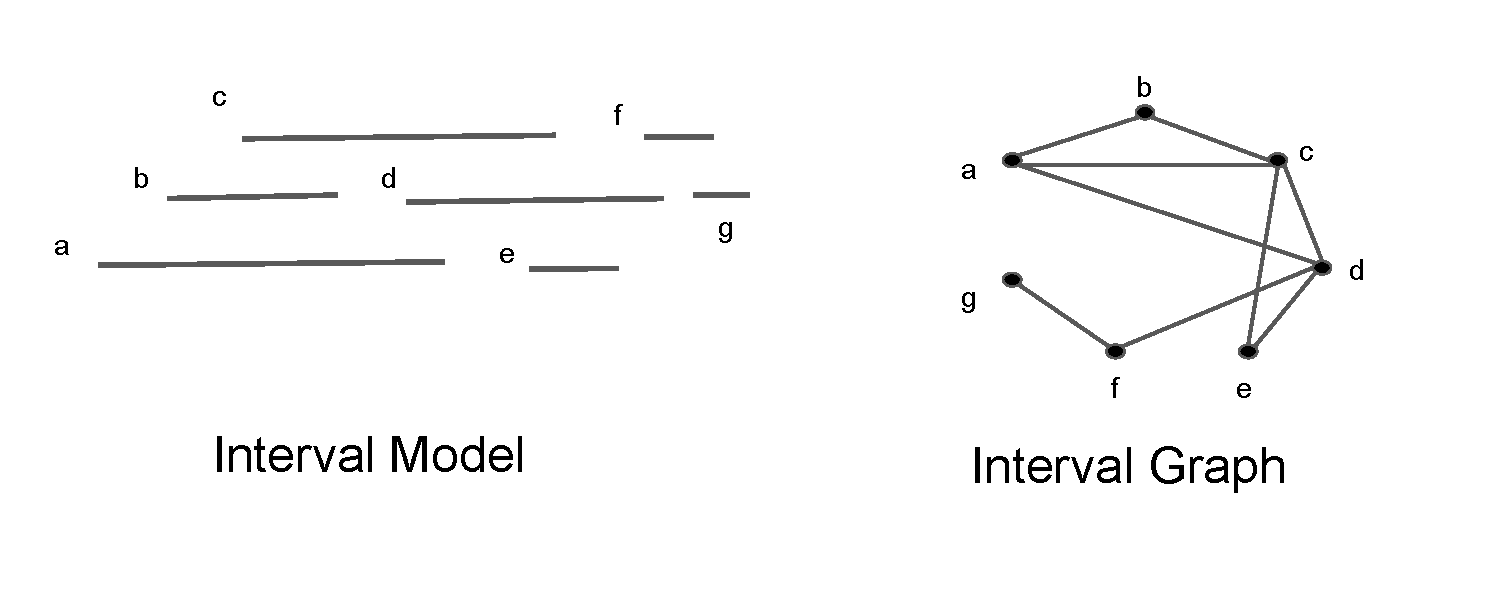
\includegraphics[width = 1.0\textwidth]{figures/interval_graph.pdf}
	\end{figure}
Applications: genetics, bioinformatics, and various resource allocations problems.
\end{frame}

\begin{frame}
	\frametitle{Chordal Graphs}
		A \emph{chordal graph} is a graph in which all cycles of four or more vertices have a chord.
		
		\vspace{0.1in}
		
		The class of interval graphs is a subclass of chordal graphs.
		
		\vspace{0.1in}
		
		Chordal graphs can be recognized in O(n+m) time using Lexicographic Breadth First Search(Lex-BFS)\footcite{rose1976algorithmic}.
		
	\begin{figure}
		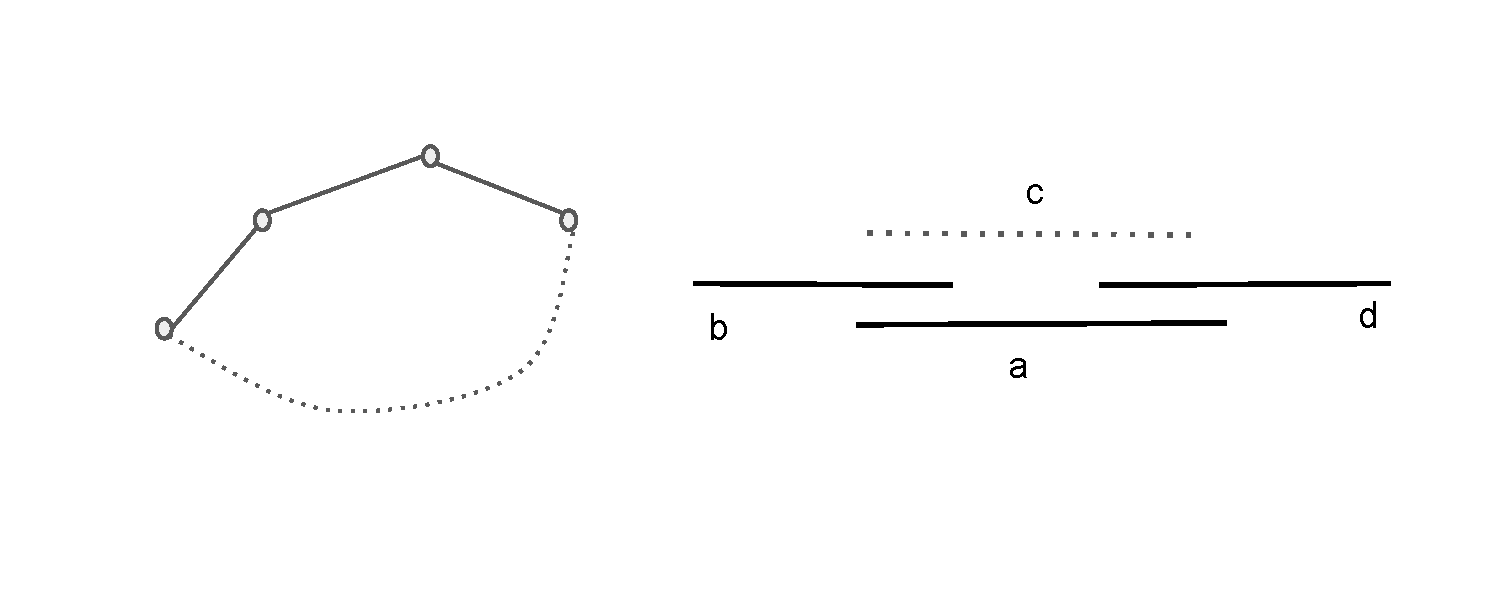
\includegraphics[width = 1\textwidth]{figures/chordal_graph.pdf}
	\end{figure}

	
\end{frame}

\begin{frame}{Outline}
\begin{itemize}
    \item Chordal Graphs and Interval Graph Characterizations
    \vspace{0.2in}
    \item Linear Time Recognition Algorithm
    \vspace{0.2in}
    \item Finding Forbidden Structures
\end{itemize}
\end{frame}
   

\begin{frame}
	\frametitle{Some Terms}
	\emph{Clique}: a subset of vertices of an undirected graph such that every two distinct vertices in the clique are adjacent.
	
	\vspace{0.1in}
	
	\emph{Maximal clique}: a clique that cannot be extended to a larger clique by including one more vertex.
	
	\vspace{0.1in}
	
	\emph{Clique Matrix}: a matrix such that the entry in row $i$ column $j$ is one if vertex $i$ is a member of clique $j$.
	
	
	\begin{figure}
		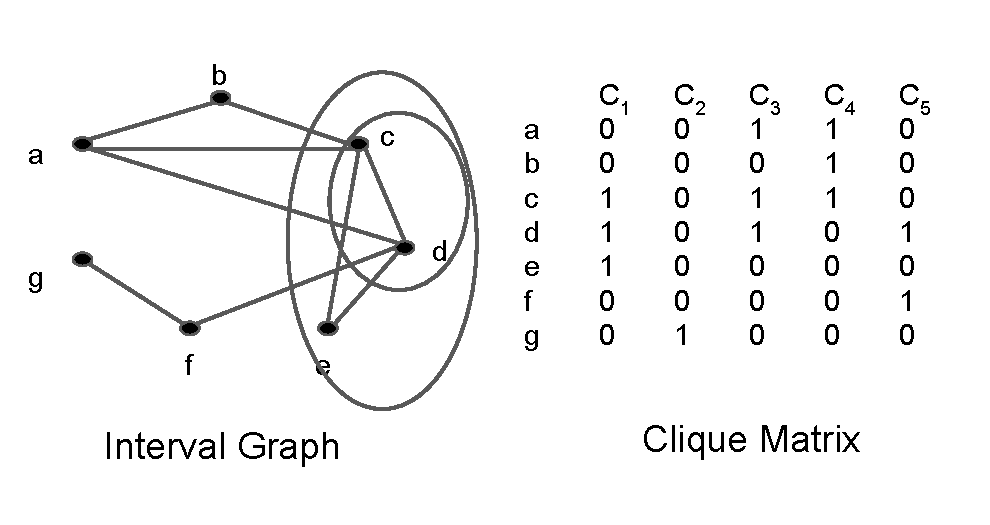
\includegraphics[width = 0.7\textwidth,height = 0.35\textheight]{figures/clique_matrix.pdf}
	\end{figure}
	Maximal cliques: $C_1: \{c,d,e\}$, $C_2: \{f,g\}$, $C_3: \{a,c,d\}$, $C_4: \{a,b,c\}$, $C_5: \{d,f\}.$
\end{frame}

\begin{frame}
	\frametitle{Some Terms}
	Simplicial Vertex: A vertex $x$ is a \emph{simplicial vertex} if its neighbors form a clique.
	    
	\vspace{0.1in}
	
	Induced Subgraph: An \emph{induced subgraph} $G_S$ is a subset $S$ of the vertices of a graph $G(V,E)$ together with any edges whose endpoints are both in $S$.
	
	
	\begin{figure}
		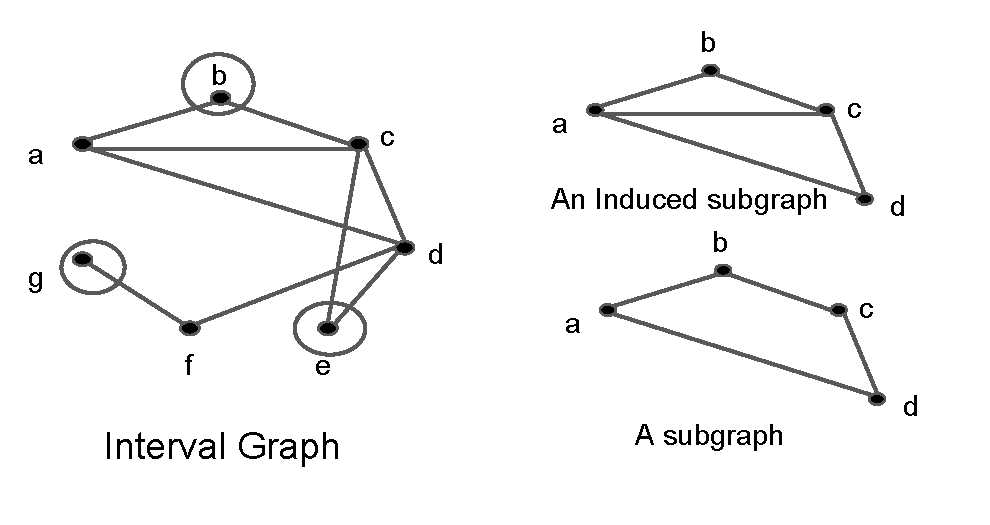
\includegraphics[width = 0.7\textwidth]{figures/simplicial_induced.pdf}
	\end{figure}

\end{frame}

\begin{frame}{Outline}
\begin{itemize}
    \item \textbf{Chordal Graphs and Interval Graph Characterizations}
    \vspace{0.2in}
    \item Linear Time Recognition Algorithm
    \vspace{0.2in}
    \item Finding Forbidden Structures
\end{itemize}
\end{frame}



%3
\begin{frame}
	\frametitle{Characterizations of Interval Graphs}
	An \emph{Asteroidal Triple(AT)} is three independent vertices such that there is a path between every two vertices that avoids any neighbor of the third vertex
    
    \vspace{0.1in}
    
    \textbf{
	A graph is an \emph{interval graph} if and only if it is chordal and does not contain an \emph{AT} \footcite{lekkerkerker1962representation}.}
	
	\begin{figure}
		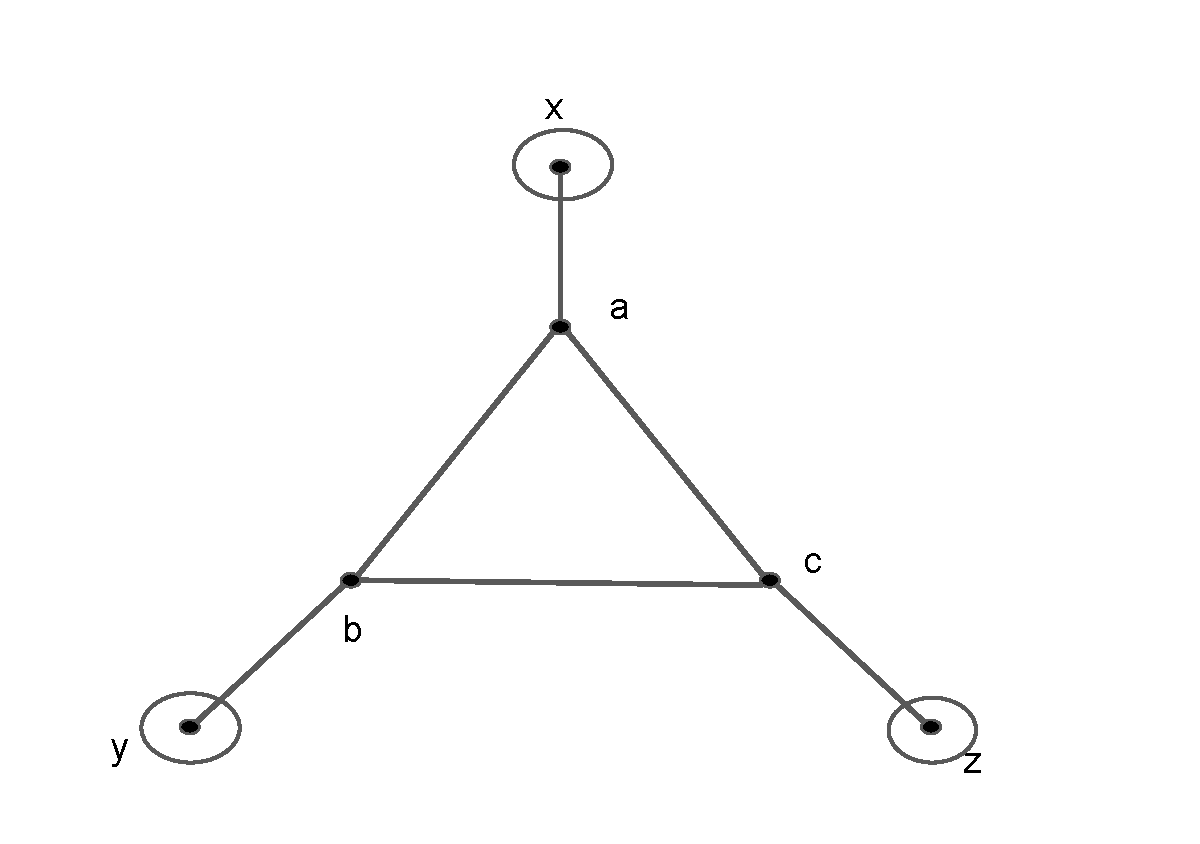
\includegraphics[height = 0.4\textheight]{figures/at.pdf}
	\end{figure}


\end{frame}

%3
\begin{frame}
	\frametitle{Characterizations of Interval Graphs}
    Lekerkerker-Boland Subgraphs: the minimal forbidden induced subgraphs for the class of interval graphs:
    \begin{figure}
		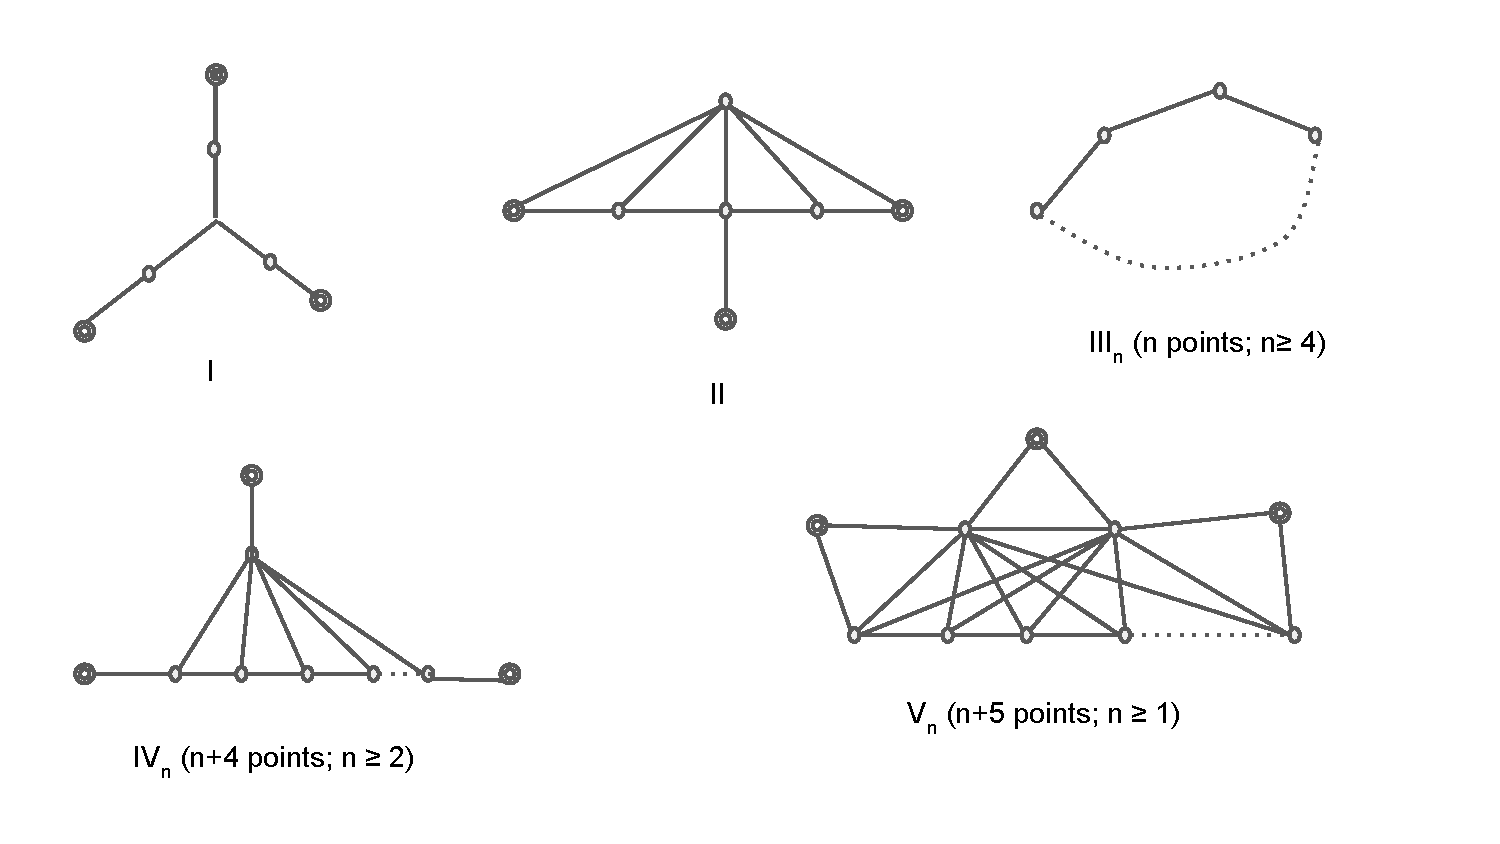
\includegraphics[width = 1.0\textwidth]{figures/lb_subgraph.pdf}
	\end{figure}
\vspace{0.2in}

\end{frame}

%5
\begin{frame}
	\frametitle{Characterizations of Interval Graphs}
	A \emph{consecutive-ones ordering} of the clique matrix is a permutation of the columns to make ones occur consecutively in each row.
    
    \vspace{0.1in}
    
    \textbf{A graph is an interval graph if and only if its clique matrix M has the consecutive-ones property\footcite{fulkerson1965incidence}.}
    
    \vspace{0.1in}
    
    Linear time recognition algorithm using PQ tree\footcite{booth1976testing}.
	\begin{figure}
		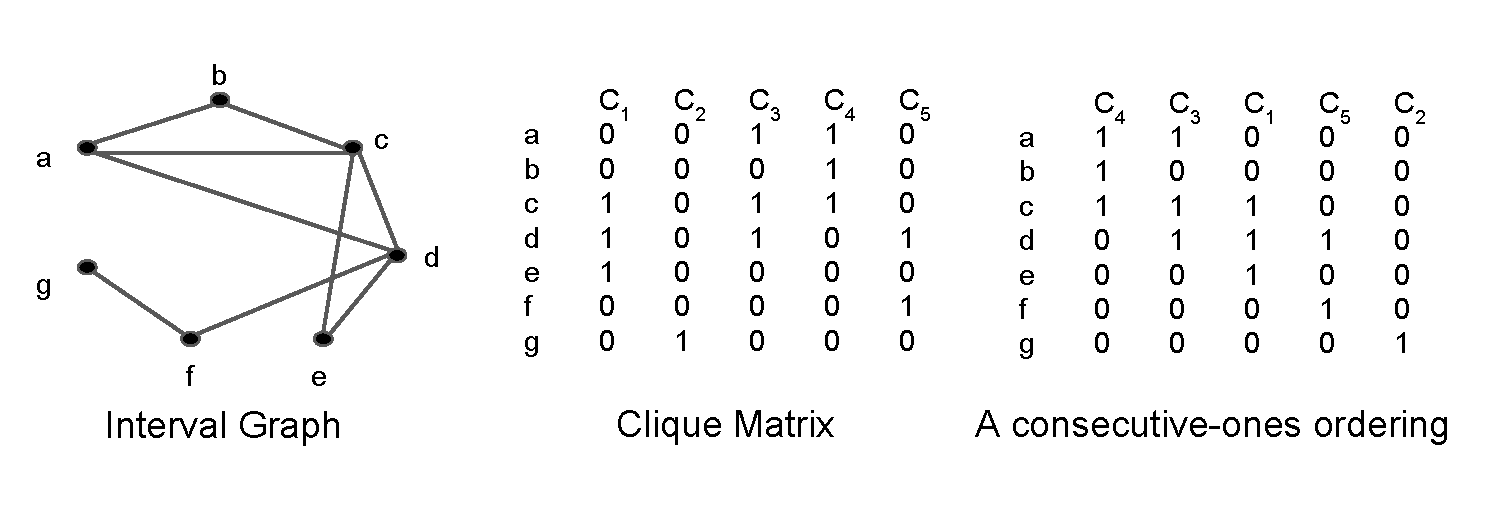
\includegraphics[width = 1\textwidth]{figures/cons_ones2.pdf}
	\end{figure}
    	
\end{frame}

%
\begin{frame}
	\frametitle{Characterizations of Interval Graphs}
	Tucker Submatrices\footcite{tucker1972structure}: forbidden submartices characterization of matrices that have consecutive-ones property:
	\begin{figure}
		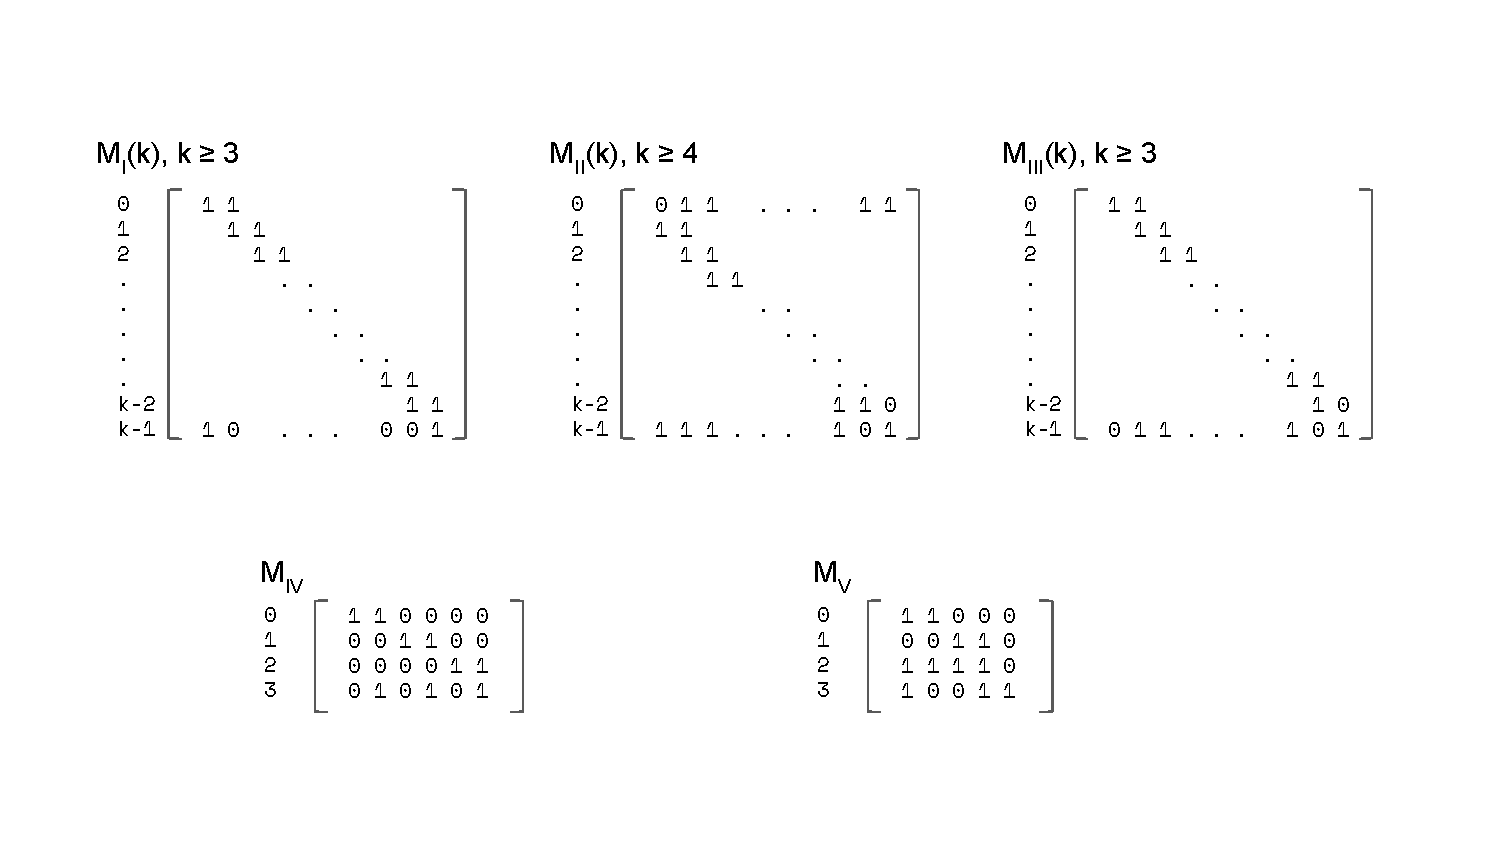
\includegraphics[width = 1\textwidth]{figures/tucker_matrix.pdf}
	\end{figure}
\end{frame}

\begin{frame}
	\frametitle{Characterizations of Interval Graphs}
	
    A graph is an \emph{interval graph} if and only if it is chordal and does not contain an \emph{Asteroidal Triple(AT)}.
	
	\vspace{0.1in}
	
	A graph is an interval graph if and only if its clique matrix M has the consecutive-ones property.
	
	\vspace{0.1in}
	
	\vspace{0.1in}
	 
	Forbidden Structures Characterizations:
	\begin{itemize}
	    \item Lekerkerker-Boland(LB) subgraphs
	    \item Tucker Submatrices
	\end{itemize}

\end{frame}

\begin{frame}{More on Chordal Graphs}
    
\begin{theorem}
Every chordal graph $G= (V,E)$ with $|V| \ge 2$ has two simplicial vertices, also, if $G$ is not a clique, the two simplicial vertices are nonadjacent.
\end{theorem}

\begin{definition}
A subset $S\in V$ is an $a-b$ \emph{vertex separator} for non-adjacent vertices $a$ and $b$ if the removal of $S$ and its adjacent edges from the subgraph separates $a$ and $b$ into different connected components. If no proper subset of $S$ is an $a-b$ separator, then $S$ is a \emph{minimal vertex separator}.
\end{definition}

\begin{lemma}
\label{lemma_separator}
Let $G$ be a chordal graph. Every minimal vertex separator is a clique in $G$.
\end{lemma}

\vspace{0.1in}

\end{frame}

\begin{frame}
	\frametitle{More on Chordal Graphs}
	
    Perfect Elimination Ordering: For a graph $G = (V, E)$, an ordering $ \sigma = [v_1, v_2, ..., v_n] $ of the vertices is a \emph{perfect elimination ordering} if every $ G_{X_i} $ for $ X_i = \{v_{j} \in N( v_{i} )|j>i\} $ is a clique.
    
    \vspace{0.1in}
    
    A graph is chordal if and only if it has a perfect elimination ordering.

	\begin{figure}
		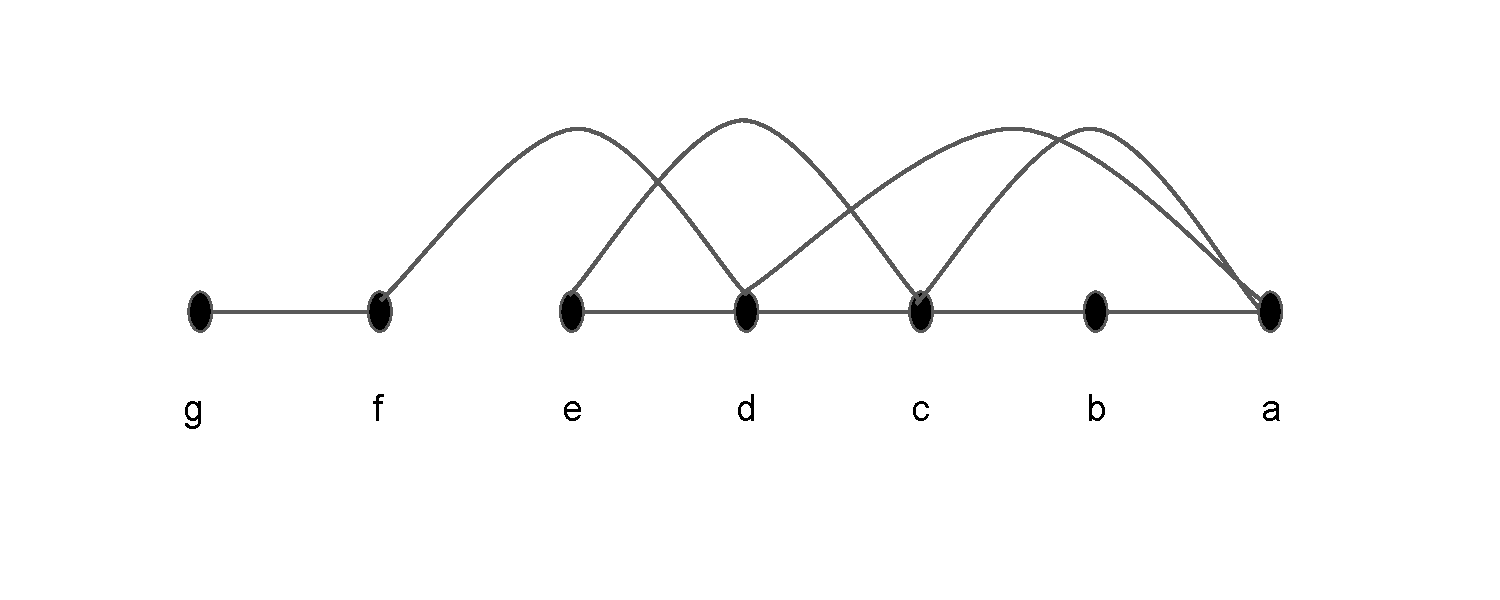
\includegraphics[width = 0.8\textwidth]{figures/peo.pdf}
	\end{figure}
	
	A valid perfect elimination ordering can be found and verified in O(n+m) time using Lexicographic Breadth First Search(Lex-BFS).
	
\end{frame}

\begin{frame}
	\frametitle{Lex-BFS}
	\begin{figure}
		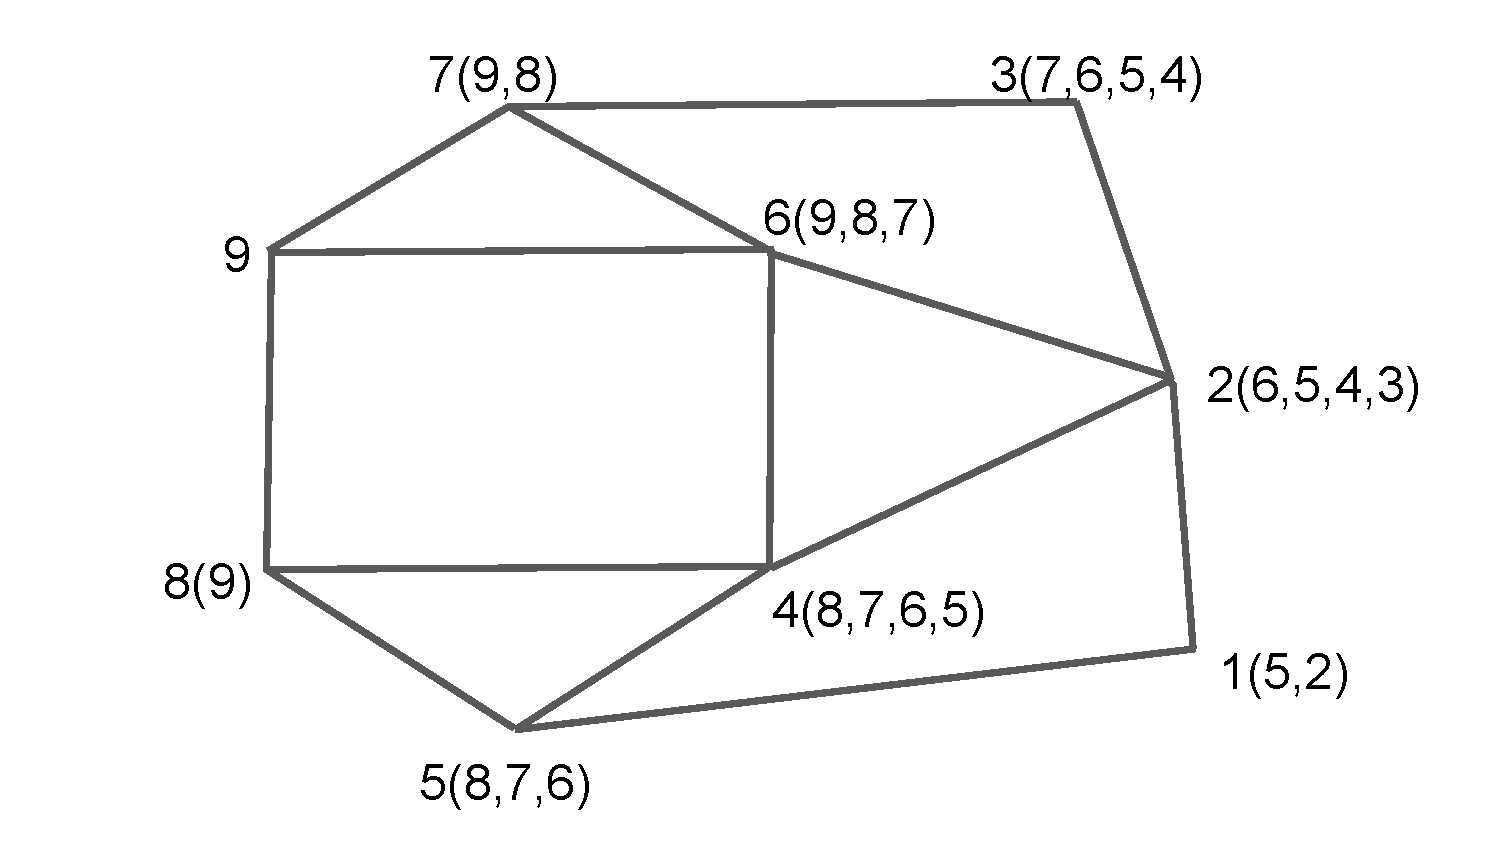
\includegraphics[width = 1\textwidth]{figures/lex_illu1.pdf}
	\end{figure}
	
\vspace{0.2in}
\end{frame}

\begin{frame}
	\frametitle{Linear Time Recognition Algorithm}
	\vspace{0.2in}
	A graph is an interval graph if and only if its clique matrix M has the consecutive-ones property.
	
	\vspace{0.2in}
	
	An arbitrary graph on n vertices can have exponential maximal cliques.
	\begin{figure}
		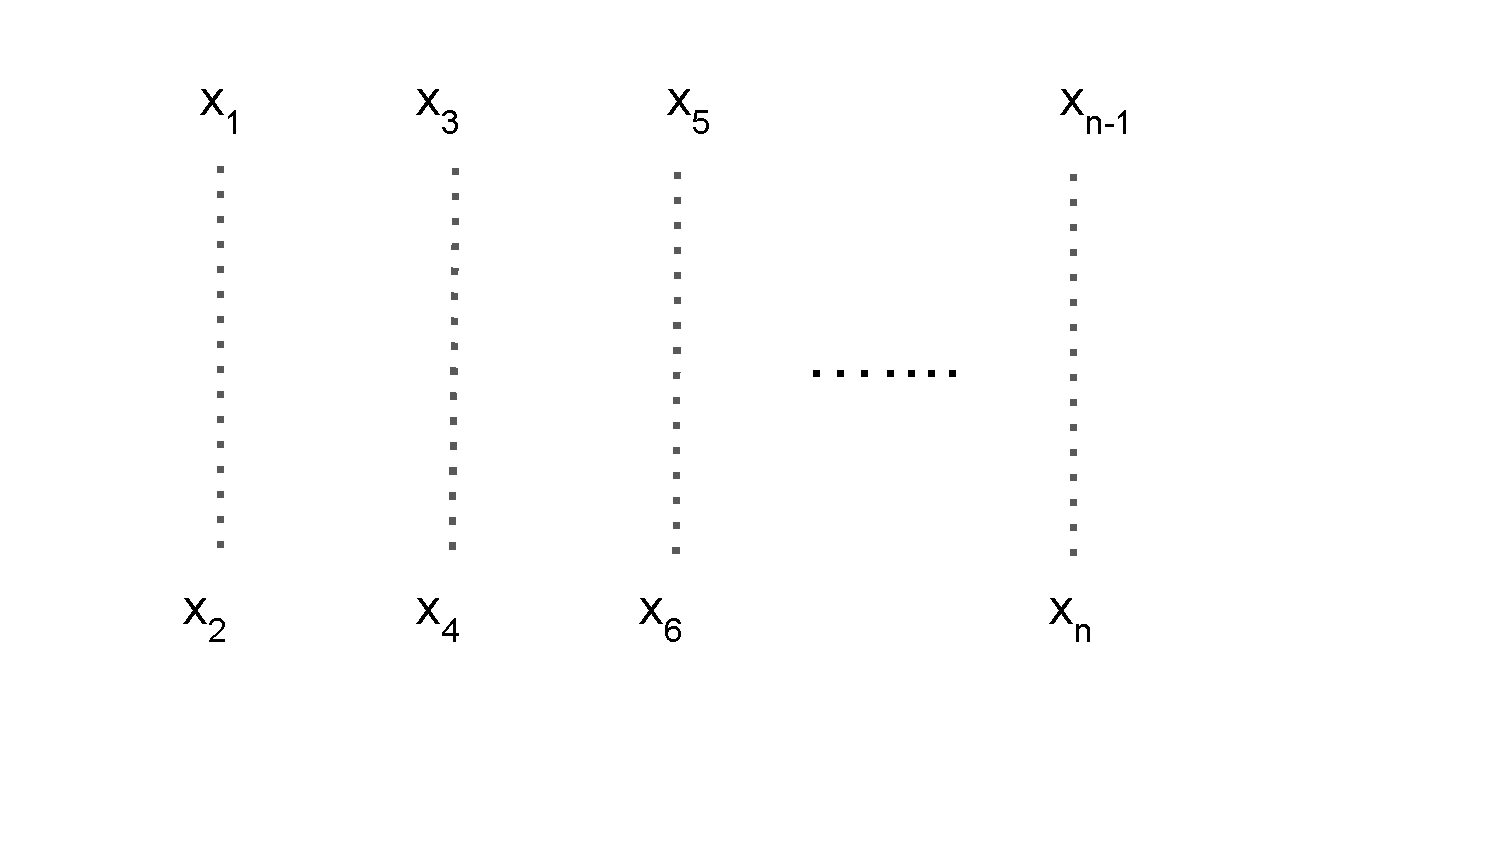
\includegraphics[width = 1\textwidth,height = 0.5\textheight]{figures/recognition_1.pdf}
	\end{figure}
	
	
\vspace{0.2in}
\end{frame}

\begin{frame}{Outline}
\begin{itemize}
    \item Chordal Graphs and Interval Graph Characterizations
    \vspace{0.2in}
    \item \textbf{Linear Time Recognition Algorithm}
    \vspace{0.2in}
    \item Finding Forbidden Structures
\end{itemize}
\end{frame}

\begin{frame}
	\frametitle{Linear Time Recognition Algorithm}
	
	For chordal graphs, the number of maximal cliques is at most $|V|$.
	
	\vspace{0.2in}
	
	Booth and Leuker's linear time recognition algorithm steps:
	\vspace{0.1in}
	
	1: Verify that G is a chordal graph, get its maximal cliques and clique matrix in $O(|V|+|E|)$ time. 
	
	\vspace{0.2in}
	
	2: Test whether or not the maximal cliques can be ordered so that those which contain vertex v occur consecutively for every $v \in V$ (using PQ-tree).
	
	
\vspace{0.2in}
\end{frame}

\begin{frame}
	\frametitle{PQ-tree}
	\vspace{0.2in}
    The PQ-tree data structure of is designed to represent a set of allowed permutations on its leaves.
    
    \vspace{0.1in}
    
    P nodes are usually denoted by circles and Q nodes by rectangles.
	\begin{figure}
		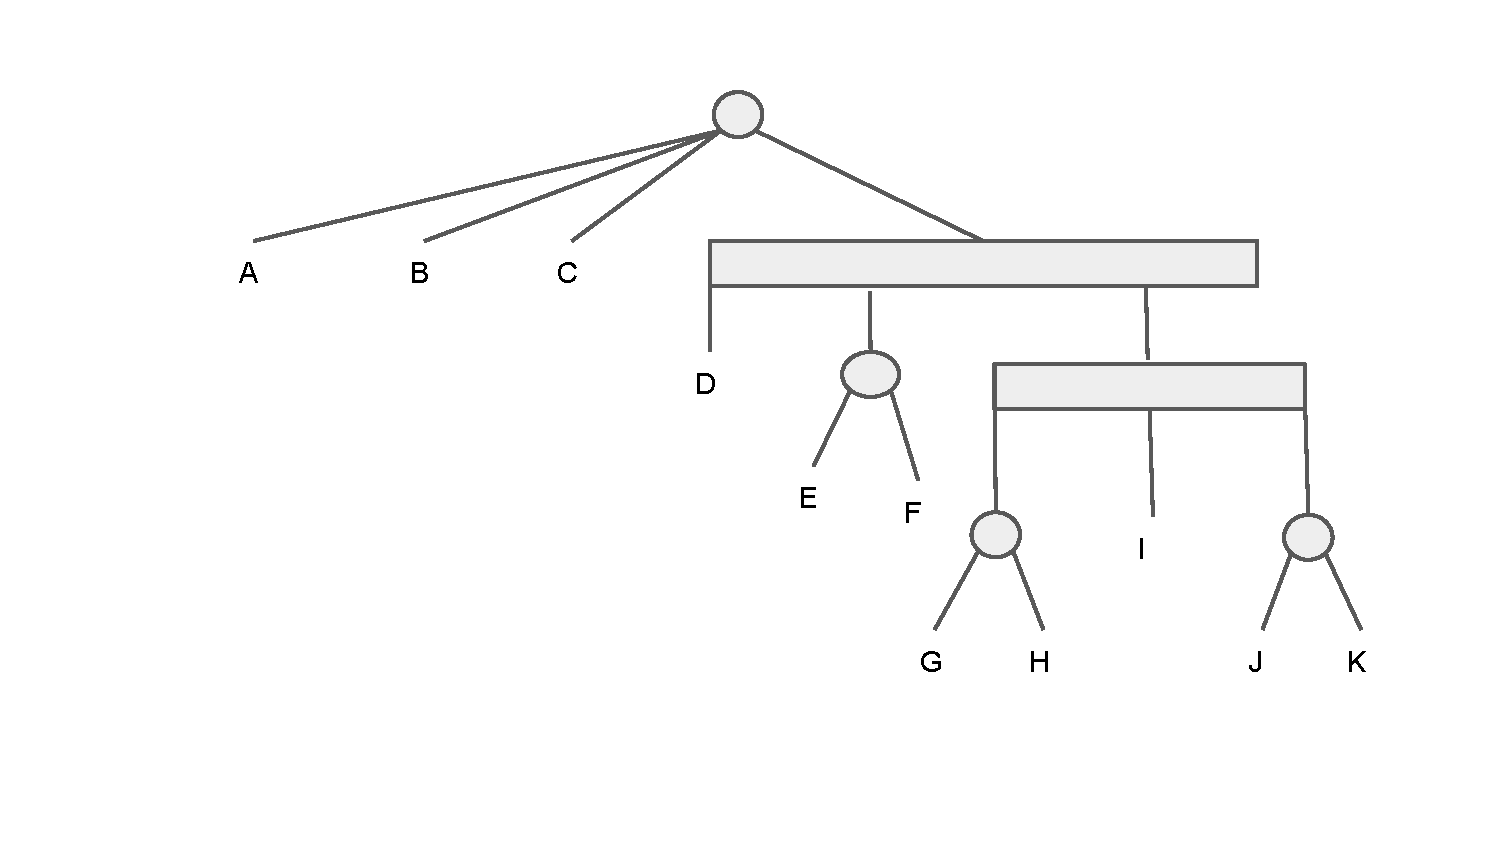
\includegraphics[width = 1\textwidth]{figures/pqtree_1.pdf}
	\end{figure}
	
\vspace{0.2in}
\end{frame}

\begin{frame}
	\frametitle{PQ-tree}
	\vspace{0.2in}
    An \emph{equivalence transform} on a PQ tree is one of the two operations below:

    \begin{enumerate}
    \item Arbitrarily permutes the order of the children of a P-node.
    \item Reverse the order of the children of a Q-node.
    \end{enumerate}
	\begin{figure}
		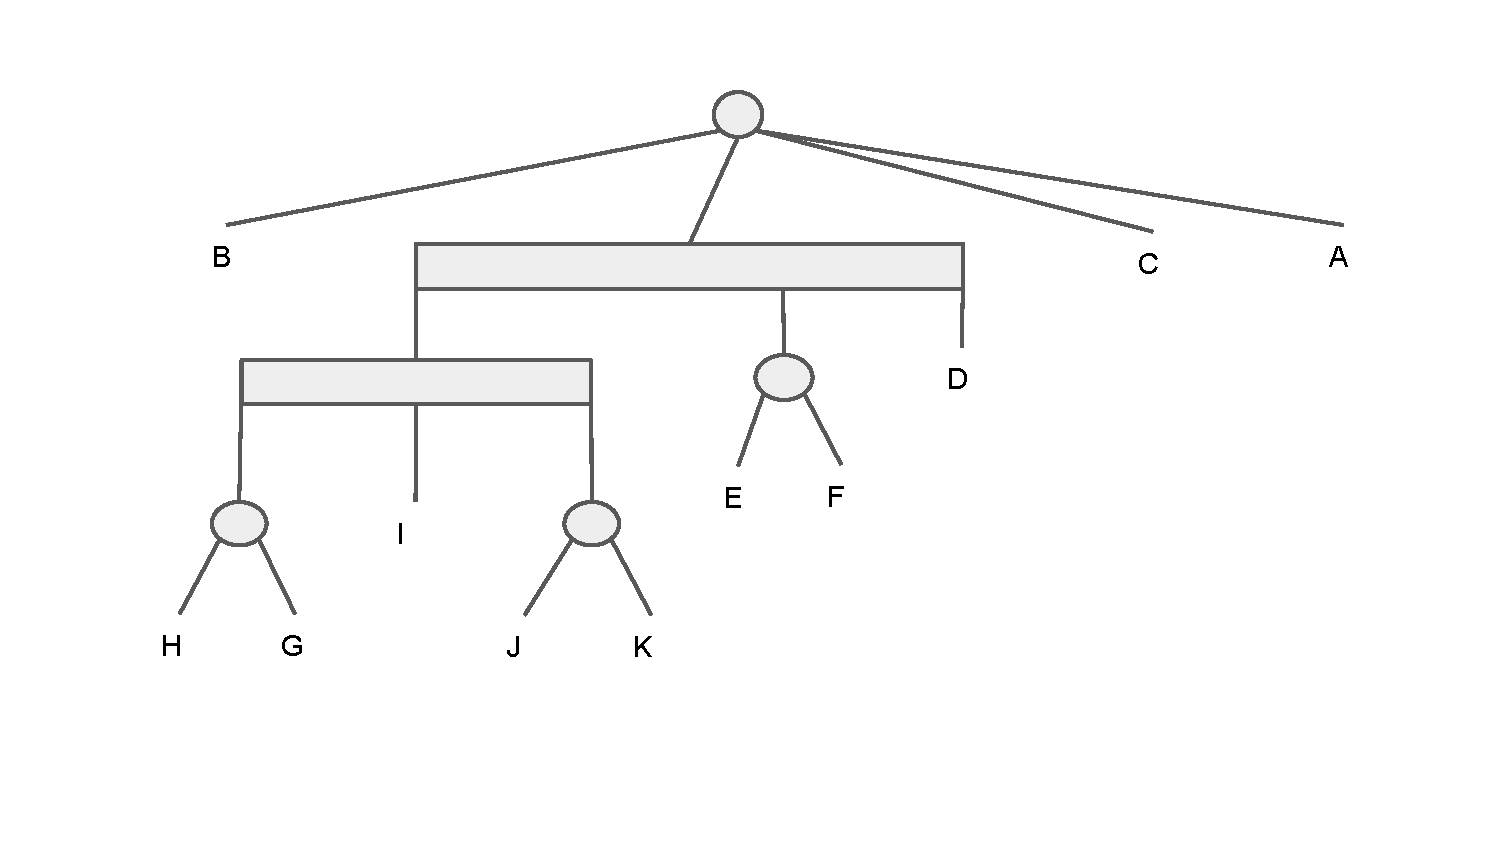
\includegraphics[width = 1\textwidth]{figures/pqtree_2.pdf}
	\end{figure}
	
\vspace{0.2in}
\end{frame}

\begin{frame}
	\frametitle{PQ-tree}
	\vspace{0.2in}
    S-reduction: selects permutations from the consistent permutations of $T$ that is consecutive for a set $S \in U$
    
    \vspace{0.1in}
    
    The returned result is either an updated a PQ-tree or we find out it is impossible to get the consecutive-ones property for this vertex.
    
    \vspace{0.1in}
    
    $S = \{ E,I,J,K\}$
    
	\begin{figure}
		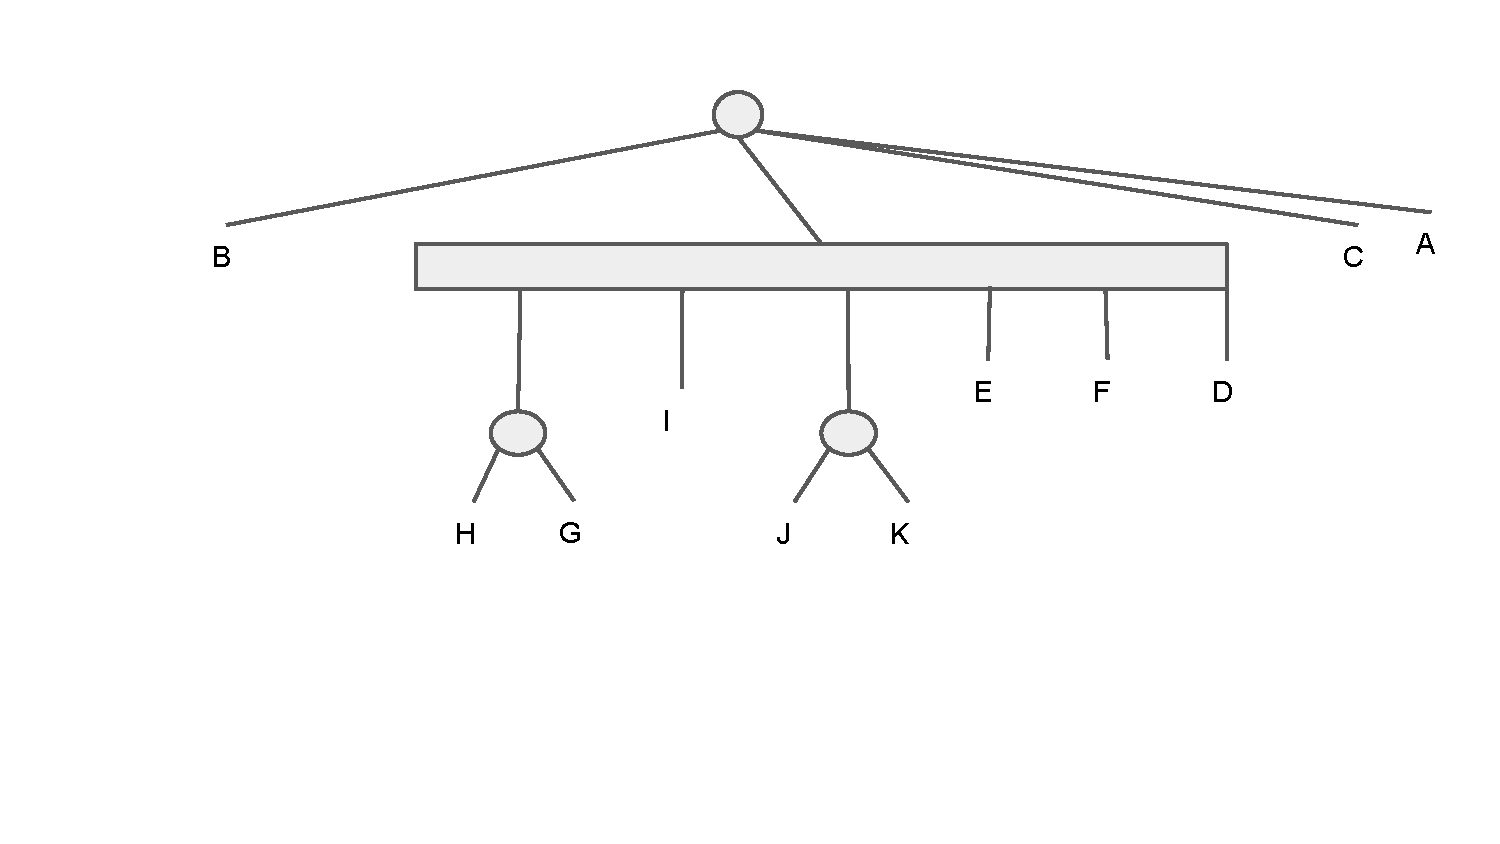
\includegraphics[width = 1\textwidth]{figures/pqtree_3.pdf}
	\end{figure}
	
\end{frame}

\begin{frame}{PQ-tree}
    Examples of Templates:
    \begin{figure}
		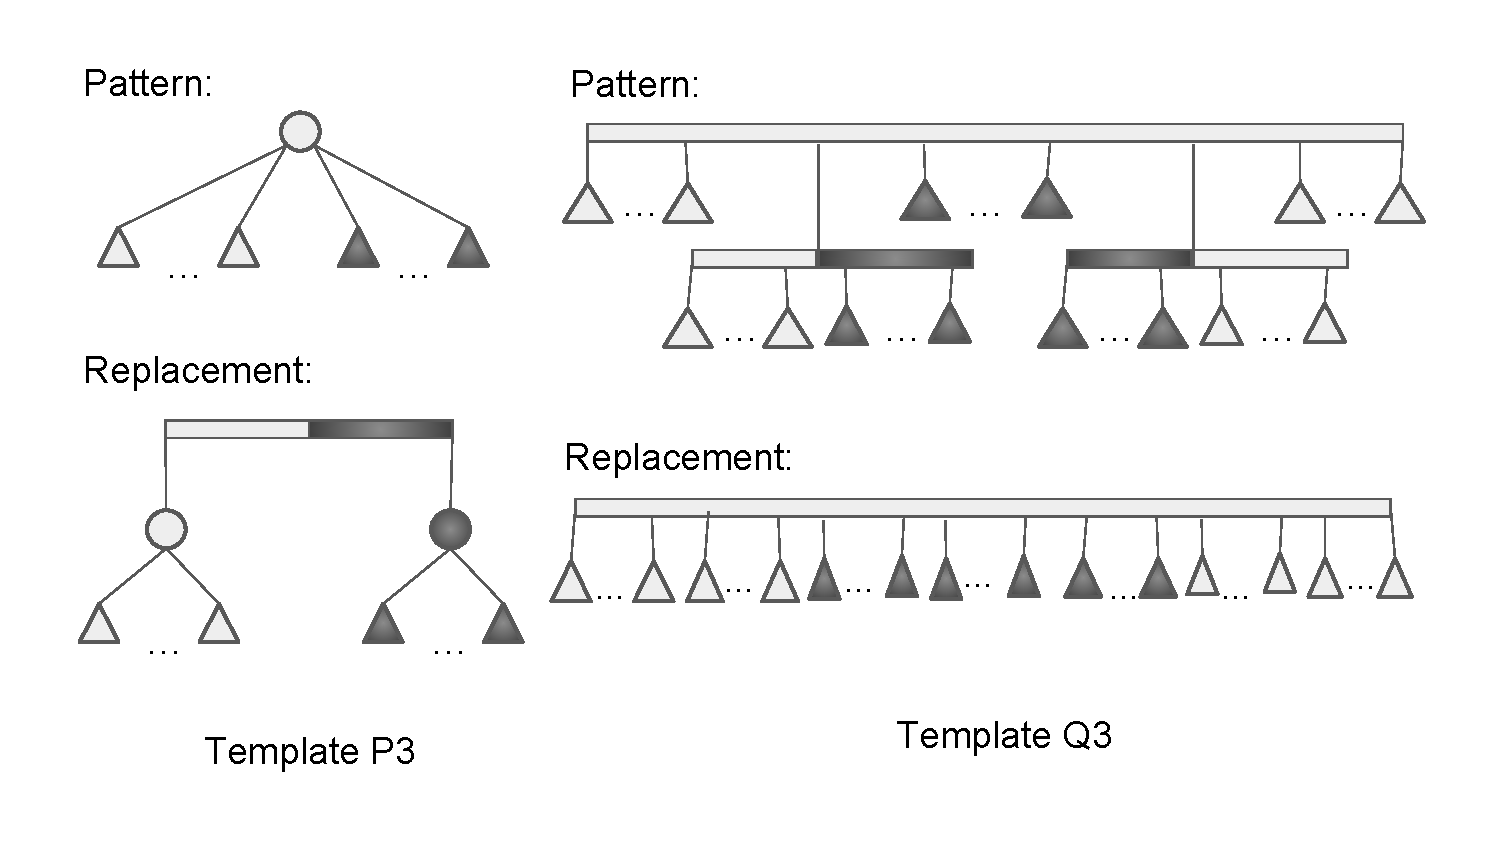
\includegraphics[width = 1\textwidth]{figures/pqtree_p3q3.pdf}
	\end{figure}
\end{frame}

\begin{frame}
	\frametitle{Linear time Recognition algorithm}
    
	\begin{figure}
		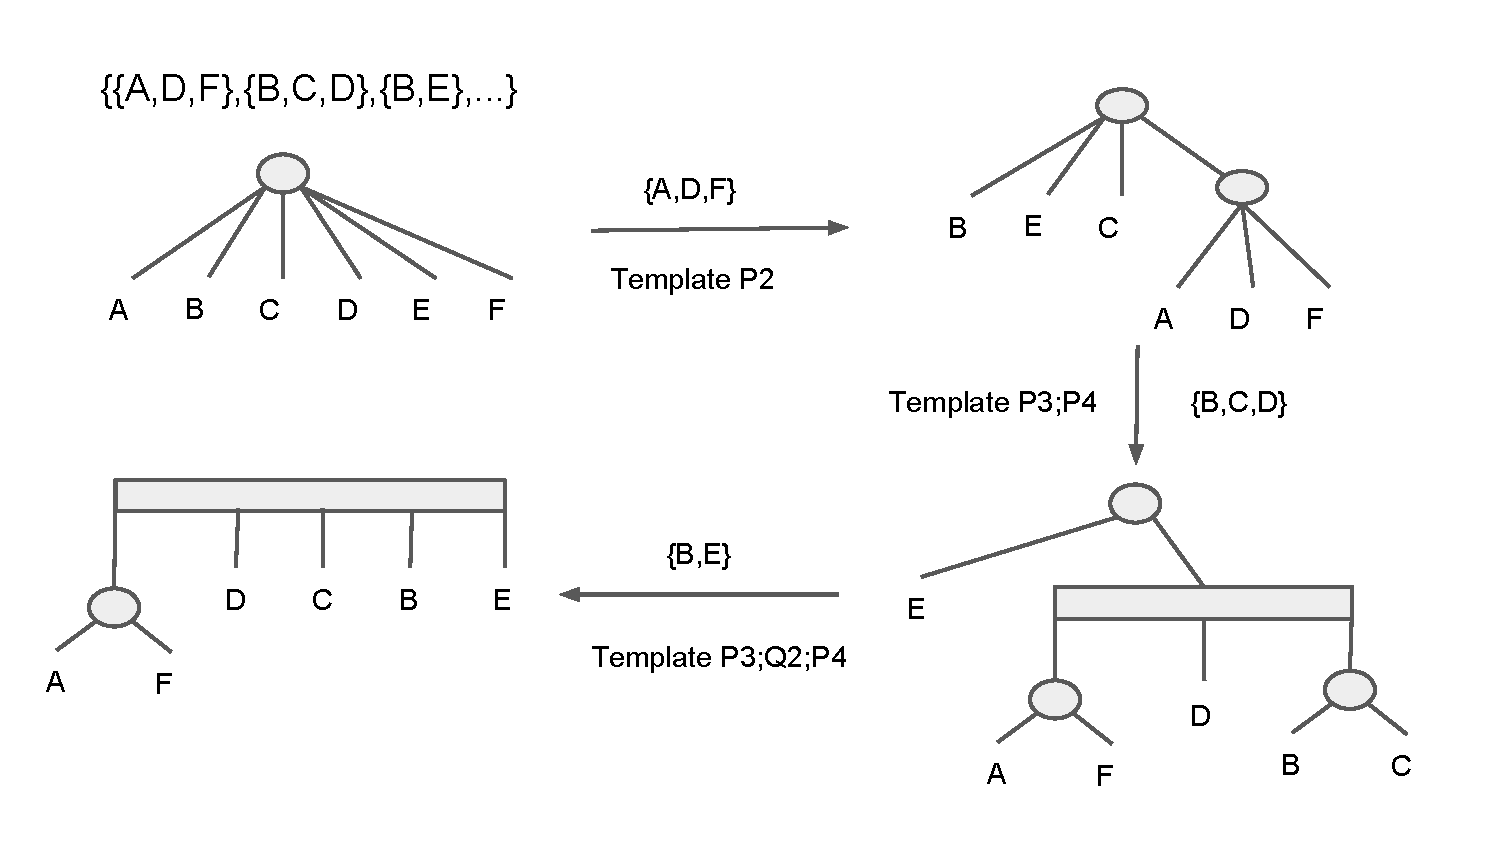
\includegraphics[width = 1\textwidth]{figures/pqtree_4.pdf}
	\end{figure}
	
\end{frame}

\begin{frame}{Outline}
\begin{itemize}
    \item Chordal Graphs and Interval Graph Characterizations
    \vspace{0.2in}
    \item Linear Time Recognition Algorithm
    \vspace{0.2in}
    \item \textbf{Finding Forbidden Structures}
\end{itemize}
\end{frame}

\begin{frame}
	\frametitle{Finding forbidden structures}
        Finding Tucker Submatrices:
	\begin{figure}
		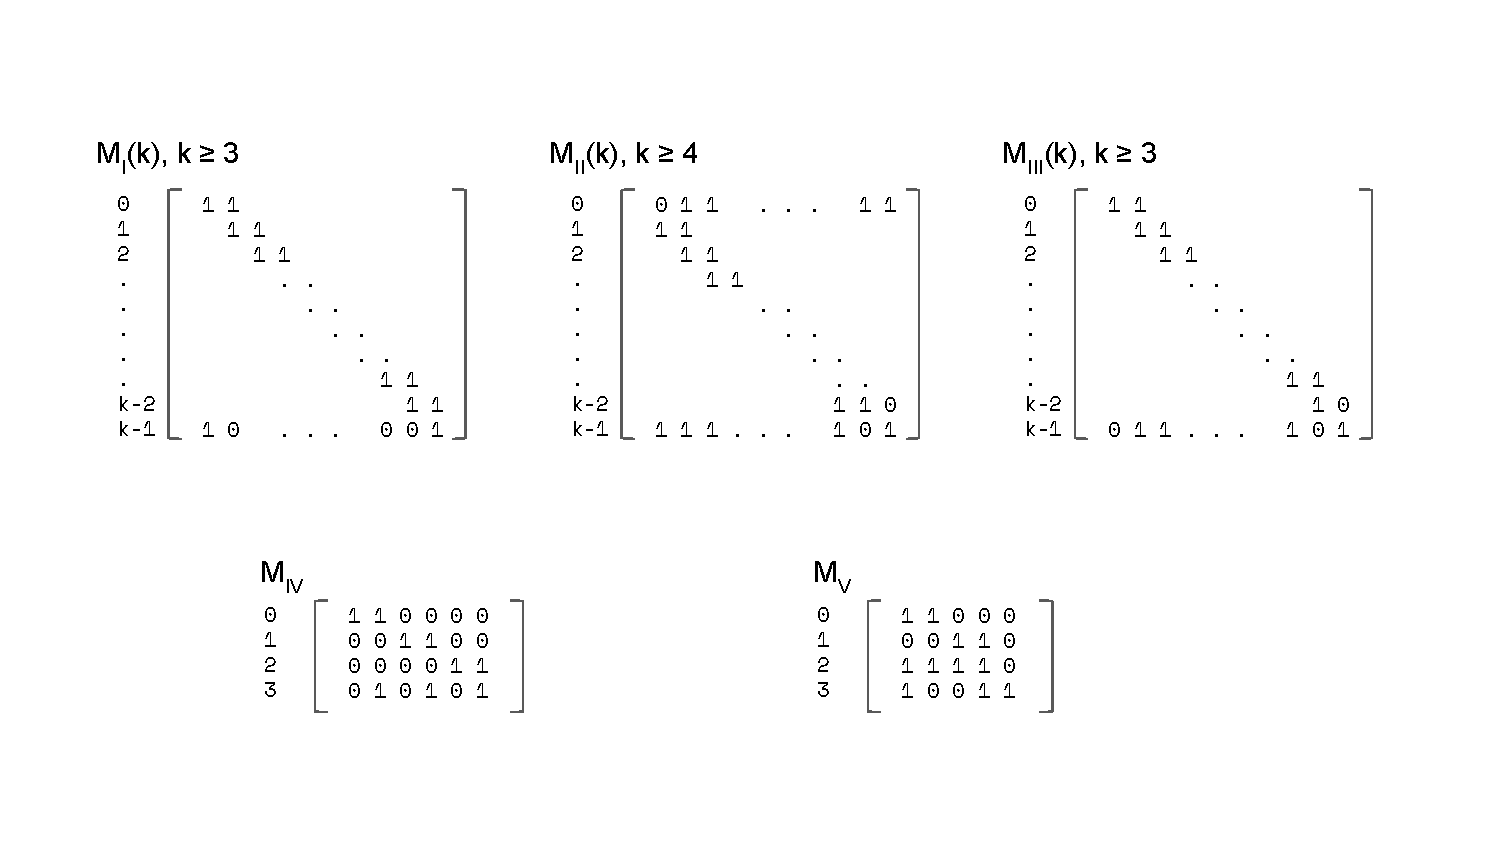
\includegraphics[width  = 1\textwidth]{figures/tucker_matrix.pdf}
	\end{figure}
	
	
\end{frame}

\begin{frame}
	\frametitle{Finding forbidden structures}
        
	\begin{figure}
		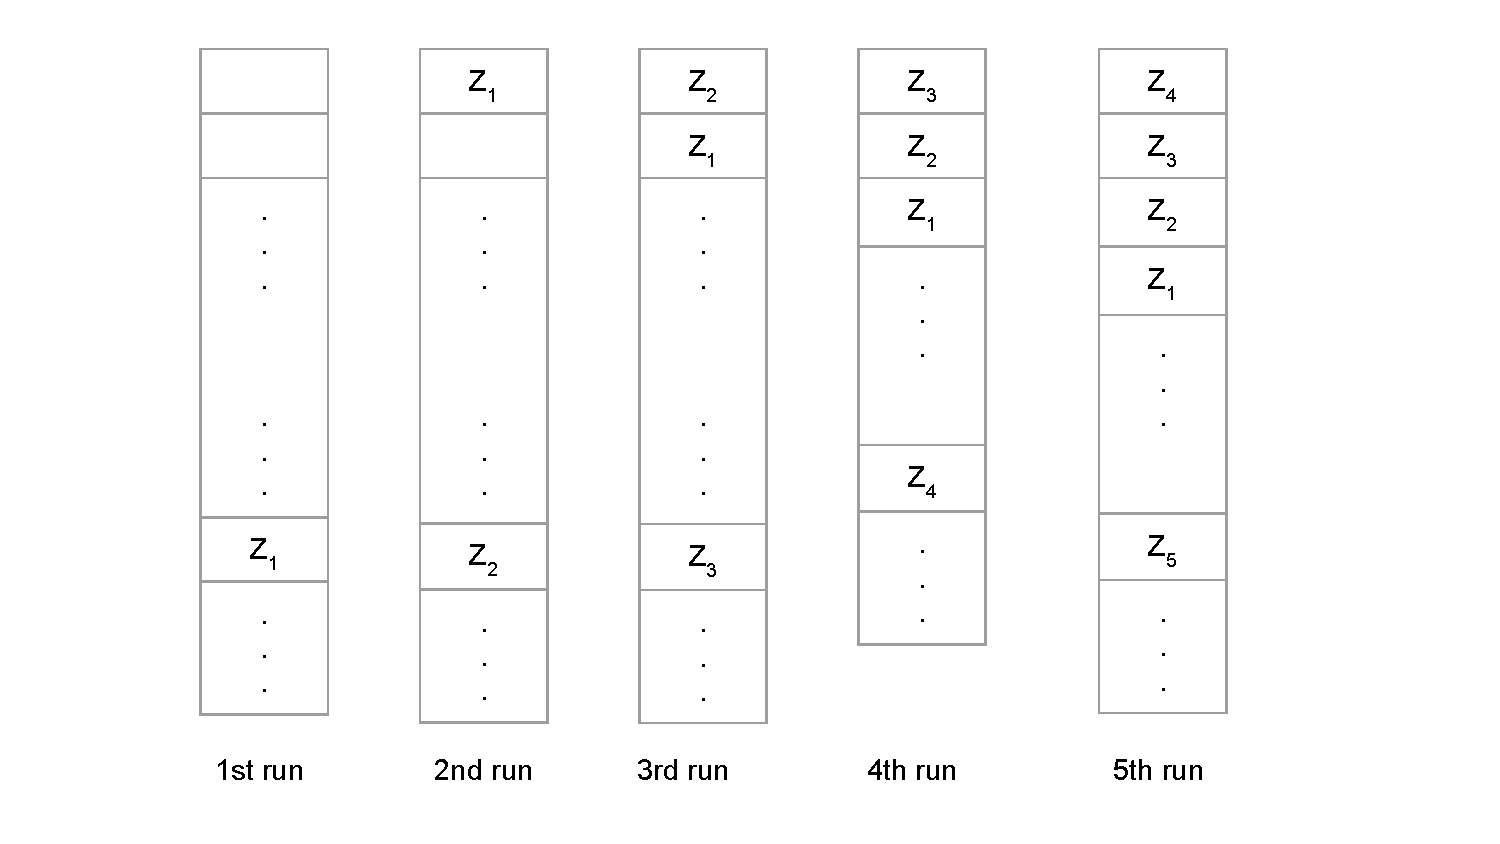
\includegraphics[width = 1\textwidth]{figures/lm_1.pdf}
	\end{figure}
	
\end{frame}

\begin{frame}
	\frametitle{Finding forbidden structures}
        
	\begin{figure}
		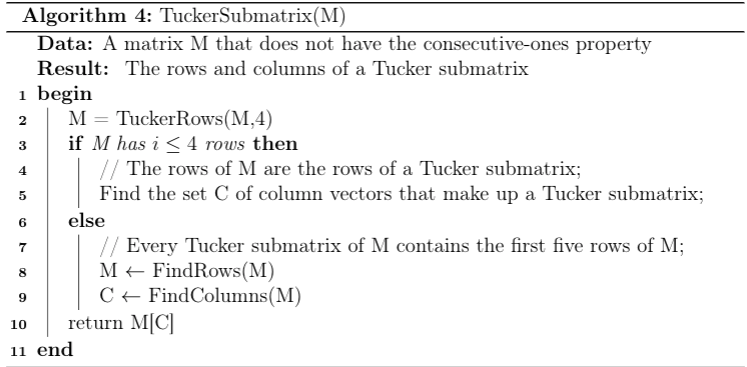
\includegraphics[width = 1\textwidth]{figures/FSalgo.png}
	\end{figure}
	
\end{frame}



\begin{frame}
	\frametitle{Finding forbidden structures}
    
    The overlap graphs of $M_I{k},M_{II}{k},M_{III}{k}$ are simple cycles.\footcite{lindzey2016linear}
    
	\begin{figure}
		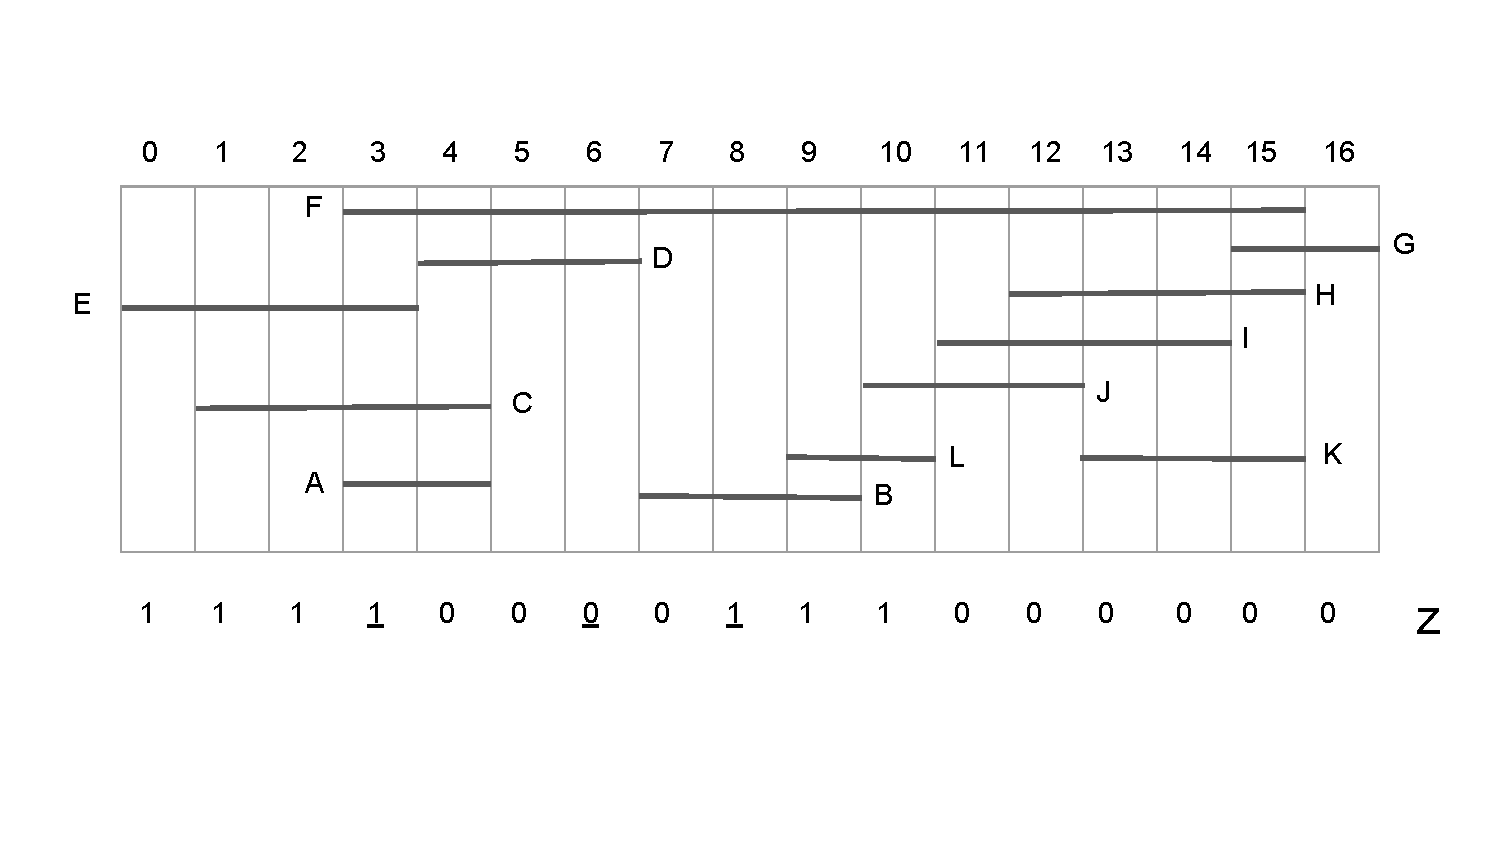
\includegraphics[width = 1\textwidth]{figures/lm_2.pdf}
	\end{figure}
	
\end{frame}
\begin{frame}
	\frametitle{Finding forbidden structures}
	\begin{figure}
		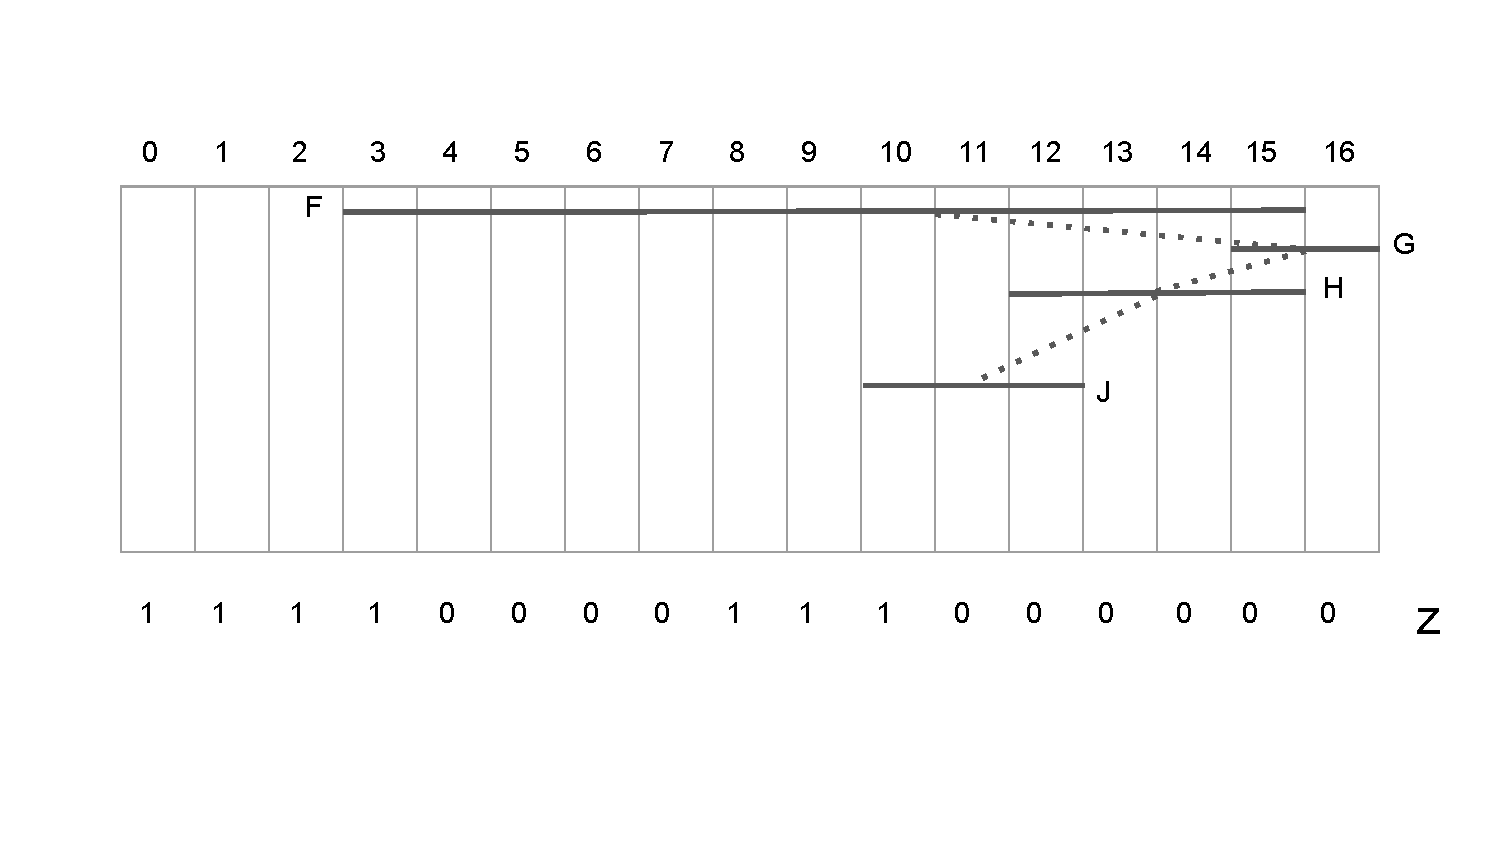
\includegraphics[width = 1\textwidth]{figures/lm_5.pdf}
	\end{figure}
	
\end{frame}

\begin{frame}[allowframebreaks]{Reference}
    \printbibliography
\end{frame}

\begin{frame}{}
  \centering \Large
  \emph{Thank you!}
\end{frame}

\begin{frame}{}
  
\end{frame}
\begin{frame}{}
  
\end{frame}
\begin{frame}{}
  
\end{frame}


\begin{frame}[allowframebreaks]{Other Characterizations}
    
    \cite{gilmore1964characterization}
    \cite{habib2000lex}
    \cite{corneil2009lbfs}
    \cite{mcconnell2009linear}
\end{frame}

\end{document}
